\begin{figure}[h]
    \centering
    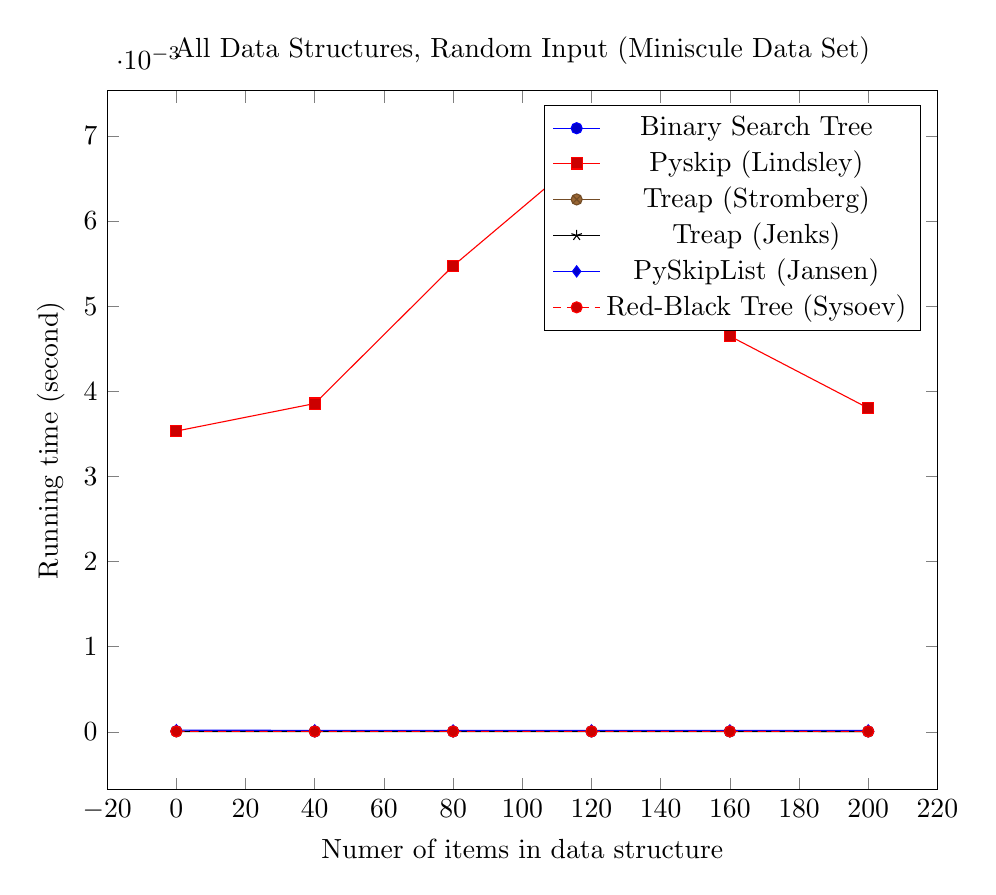
\begin{tikzpicture}
        \begin{axis}[
            xlabel={Numer of items in data structure},
            ylabel={Running time (second)},
            title={All Data Structures, Random Input (Miniscule Data Set)},
            width=\textwidth
        ]
		\addplot coordinates {
			(0, 8.101616558597869e-06)
			(40, 4.788687854340168e-06)
			(80, 4.758570320673172e-06)
			(120, 4.7886878543845764e-06)
			(160, 5.029628123764951e-06)
			(200, 4.939275522719555e-06)
		};
		\addplot coordinates {
			(0, 0.0035322747020246404)
			(40, 0.003855646661094925)
			(80, 0.0054719643408401185)
			(120, 0.006842462710728592)
			(160, 0.004647436621415091)
			(200, 0.0038015856881480127)
		};
		\addplot coordinates {
			(0, 5.360920994190721e-06)
			(40, 6.023506735042261e-06)
			(80, 4.96939305643096e-06)
			(120, 6.0837418023762526e-06)
			(160, 5.059745657431947e-06)
			(200, 4.4875125176258026e-06)
		};
		\addplot coordinates {
			(0, 2.8009306317855477e-06)
			(40, 2.3190500929803904e-06)
			(80, 2.168462424601003e-06)
			(120, 2.288932559313395e-06)
			(160, 2.108227357267012e-06)
			(200, 2.1383448909340075e-06)
		};
		\addplot coordinates {
			(0, 1.9576396888876246e-05)
			(40, 1.743805199789783e-05)
			(80, 1.629358571828554e-05)
			(120, 1.6986288992759668e-05)
			(160, 1.6745348723379295e-05)
			(200, 1.716699419485046e-05)
		};
		\addplot coordinates {
			(0, 5.692213864616491e-06)
			(40, 4.8489229217185684e-06)
			(80, 4.879040455385564e-06)
			(120, 5.150098258432933e-06)
			(160, 5.30068592685673e-06)
			(200, 4.879040455385564e-06)
		};
        \legend{Binary Search Tree, Pyskip (Lindsley), Treap (Stromberg), Treap (Jenks), PySkipList (Jansen), Red-Black Tree (Sysoev)}
        \end{axis}
    \end{tikzpicture}
    \caption{Average of 10 operations, benchmarked every 40, starting at 0.}
\end{figure}